\section{Structural Dynamics}
\label{sec:structural}

Our goal is to bound the runtime cost of evaluating a program (in our language) on a $p$ processor machine. For this purpose, we define two separate structural (small step) cost dynamics for our language: the \emph{idealized parallel dynamics} and the \emph{interleaved dynamics}.

The parallel dynamics defines the parallel \emph{span} (or depth) of a
computation, which is intuitively the number of parallel steps
given an unbounded number of processors. It is a pure dynamics
and allows all parallel expressions to proceed on the same step.

The interleaved dynamics defines the total \emph{work} performed by a
computation, which can be thought of as the number of instructions
used by the computation (within constant factors). The dynamics is
not pure, requiring a store to keep track whether each sequence is a leaf or interior, so that different costs can be charged for \get{} and \set{} in the two cases.  To account for parallelism, the dynamics allows for non-deterministic interleaving of steps on parallel expressions.  In conjunction with the impure cost for \get{} and \set{}, this means the overall work is non-deterministic. In Section~\ref{sec:evaluational} we give a deterministic cost dynamics and
show that it provides an upper bound on the work over all possible
interleavings.

The two dynamics are useful together because we can bound the
runtime on any fixed number of processors based on the work and span.

\subsection{Idealized Parallel Dynamics}

The idealized parallel dynamics captures the evaluation steps taken on a
machine with an unbounded number of processors and
is given by the following judgement, where $e$ is the expression and
$e'$ is the resulting expression:
$$e \to_{par} e'$$

Let $\overline{\text{\get{}}}(A, i)$ denote $A[i]$, $\overline{\text{\set{}}}(A, (i,v))$ denote $A[i \mapsto v]$ (which denotes the sequence obtained if the value at index $i$ of $A$ is replaced with $v$), and $\overline{\text{\new{}}}((n,v))$ denote a sequence of size $n$ with the value $v$ at each index. Intuitively, $\overline{\text{\get{}}}$, $\overline{\text{\set{}}}$, and $\overline{\text{\new{}}}$ represent abstract versions of \get{}, \set{}, and \new{}.

We show the rules for get and fork-join in Figure \ref{fig:parallel-dynamics}. As usual, the judgement \func{val} describes terminal values. Notice that in fork-join, both sides of the fork-join take a step at the same time if possible. The rules for \set{} and \new{} are similar to the rules for \get{}, and the rules for function application and if-then are as in a standard applicative order functional programming language. 

\begin{figure}
$$\frac{A, a \; \text{val}}{\tget{}(A, a) \to_{par} \overline{\mbox{\get{}}}(A, a)} \text{ (get-eval)}$$
$$\frac{e_1 \to_{par} e_1' \;\;\; e_2 \to_{par} e_2'}{e_1 || e_2 \to_{par} e_1' || e_2'} \text{ (fork)}$$
$$\frac{v_1 \; \text{val} \;\;\; e_2 \to_{par} e_2'}{v_1 || e_2 \to_{par} v_1 || e_2'} \text{ (step-right)}$$
$$\frac{v_2 \; \text{val} \;\;\; e_1 \to_{par} e_1'}{e_1 || v_2 \to_{par} e_1' || v_2} \text{ (step-left)}$$
$$\frac{v_1, v_2 \text{ val}}{(v_1 || v_2) \to_{par} (v_1, v_2)} \text{ (join)}$$

\caption{Example rules in the parallel dynamics for our language.}
\label{fig:parallel-dynamics}
\end{figure}

The parallel structural dynamics, unlike the interleaved
structural dynamics, is deterministic.

\begin{definition}
A \emph{parallel transition sequence} $T$ is a sequence $(e_0, ..., e_n)$ with $e_i \to_{par} e_{i+1}$ for all $0 \leq i < n$. We say that $e_0 \to^n_{par} e_n$ or $e_0 \to^*_{par} e_n$.
\end{definition}

\begin{definition}
The \emph{span} of a parallel transition sequence $T$, denoted by $SP(T)$, is its length $n$.
\end{definition}

\subsection{Interleaved Cost Dynamics}

The interleaved dynamics is a concurrent dynamics and is given by the following judgement, where $\sigma$ is the
store, $e$ is the expression, $\sigma'$ is the resulting store, $e'$ is the
resulting expression after a step has been taken, and $w$ is the work.
$$\sigma, e \to \sigma', e', w$$

Sequence values are represented by the pair $(l, V)$ where $l$ is a
label into the store $\sigma$ and $V$ is a list of the elements in the sequence.  The store is a mapping from labels to either $+$ (indicating a leaf sequence)
or $-$ (indicating an interior sequence). Let $L(\sigma)$ denote the set of labels in the store $\sigma$.

Let $g_l(V)$ and $g_i(V)$ be the work of \get{} applied to $V$ if it
is a leaf or interior sequence, respectively, and $s_l(V)$ and $s_i(V)$
be the work of \set{} applied to $V$ if it is a leaf or interior
sequence.  Let $n(a)$ be the work of evaluating \new{}$(a)$.  We assume
that $g_l(V) \leq g_i(V)$ and $s_l(V) \leq s_i(V)$ (operating on leaf
sequences is cheaper that operating on interior sequences).

\begin{figure}
$$\frac{v_1, v_2 \; \text{val}}{\sigma, (\lambda (x,y).e)(v_1,v_2) \to \sigma, [v_1/x][v_2/y]e, 1} \text{ (func-app)}$$

$$\frac{}{\sigma, \text{if } \text{true} \; e_2 \; e_3 \to \sigma, e_2, 1} \text{ (if-true)}$$

$$\frac{}{\sigma, \text{if } \text{false} \; e_2 \; e_3 \to \sigma, e_3, 1}  \text{ (if-false)}$$

$$\frac{a \; \text{val} \;\;\; l \not\in L(\sigma)}{\sigma, \tnew{}(a) \to \sigma[l \mapsto +], \overline{\mbox{\new{}}}(a), n(a)} \text{ (new)}$$

$$\frac{A = (l, V) \;\;\; \sigma[l] = + \;\;\; a \text{ val}}{\sigma, \tget{}(A, a) \to \sigma, \overline{\mbox{\get{}}}(V,a), g_l(V)} \text{ (get-leaf)}$$

$$\frac{A = (l, V) \;\;\; \sigma[l] = -  \;\;\; a \text{ val}}{\sigma, \tget(A, a) \to \sigma, \overline{\mbox{\get{}}}(V,a), g_i(V)} \text{ (get-interior)}$$

$$\frac{A = (l, V) \;\;\; \sigma[l] = + \;\;\;  l' \not\in L(\sigma) \;\;\; a \text{ val}}{\begin{gathered}\sigma, \tset(A, a) \to \sigma[l \mapsto -, l' \mapsto +], \\ (l', \overline{\mbox{\set{}}}(V, a)), s_l(V)\end{gathered}} \text{ (set-leaf)}$$

$$\frac{A = (l, V) \;\;\; \sigma[l] = - \;\;\;  l' \not\in L(\sigma) \;\;\; a \text{ val}}{\begin{gathered}\sigma, \tset(A, a) \to \sigma[l' \mapsto +], \\ (l', \overline{\mbox{\set{}}}(V,a)), s_i(V)\end{gathered}} \text{ (set-interior)}$$

$$\frac{\sigma, e_1 \to \sigma', e_1', w}{\sigma, e_1 || e_2 \to \sigma', e_1' || e_2, w} \text{ (step-left)}$$
$$\frac{\sigma, e_2 \to \sigma', e_2', w}{\sigma, e_1 || e_2 \to \sigma', e_1 || e_2', w} \text{ (step-right)}$$
$$\frac{v_1, v_2 \text{ val}}{\sigma, (v_1 || v_2) \to \sigma, (v_1, v_2), 1} \text{ (join)}$$

\caption{The interleaved dynamics for our language.  We omit
  rules that involve stepping the arguments to \get{}, \set{}, \new{},
  and other language constructs.}
\label{fig:interleaved}
\end{figure}

The dynamics is given in figure~\ref{fig:interleaved}.  Note that
\set$(A,a)$ where $A = (l,V)$ and $\sigma[l] = +$ creates a new label and
value, extends the store to indicate the new value is a leaf, and
updates the store at $l$ to indicate that $A$ is now interior.  This
is the impure aspect of the cost dynamics since there can be other
references to $l$.  Also note that the work for for \get{} and \set{}
depends on whether the sequence is a leaf or interior.

The rules for fork-join are non-deterministic---either side of the
fork can take a step.  This allows for arbitrary interleaving of
instructions on different sides of a fork-join.  After both sides of a
fork-join are fully evaluated the parallel pair is converted to a regular pair.

\begin{definition}
A \emph{transition sequence} $T$ is a sequence of states $[(\sigma_0, e_0),
..., (\sigma_n, e_n)]$ and per-step work $[w_1, ..., w_n]$ s.t. for all $0 \leq i < n$, $\sigma_i, e_i \to \sigma_{i+1}, e_{i+1}, w_{i+1}$ . We say that $T$ takes $\sigma_0, e_0$ to $\sigma_n, e_n$ and has length $n$ and denote this by $\sigma_0, e_0 \to^n \sigma_n, e_n$.
\end{definition}

\begin{definition}
We say that $T$ is \emph{maximal} if there does not exist $\sigma', e', w'$ s.t. $\sigma_n, e_n \to \sigma', e', w'$.
\end{definition}

\begin{definition}
A \emph{transition subsequence} $T_{i, j}$ of $T$ is given by the
sequence of states $[(\sigma_i, e_i), ..., (\sigma_j, e_j)]$ and per-step work
$[w_{i+1}, ..., w_j]$. Note that $T = T_{0,n}$.   
\end{definition}

\begin{definition}
The \emph{work of a transition sequence} $T$ is given by:
$$W(T) = \sum_{i=1}^n w_i$$
\end{definition}

Different transition sequences starting and ending at the same states
may have different work.  In particular, a sequence can be used
concurrently by multiple parallel expressions and the work could
depend on the order in which the instructions are interleaved.
Figure~\ref{fig:fork_join_intuition} shows 3 ways a leaf sequence $A$
might be used.  In particular, one side of the fork might call \get{}
on $A$ while the other side calls \set{} (see the center panel). Calls
to \get{} on the left branch would have work $g_l(A)$ if and only if
they execute before the call to \set{} on the right branch, otherwise
they would have work $g_i(A)$.

\begin{figure}[!ht]
\centering
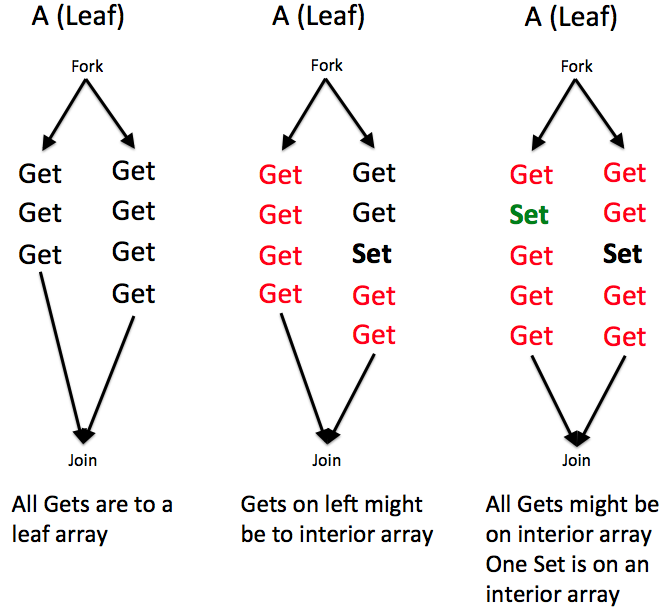
\includegraphics[scale=0.3]{fork_join_intuition}
\nocaptionrule \caption{Different ways a sequence might be used in a fork join}
\label{fig:fork_join_intuition}
\end{figure}

We cannot make any assumptions about how the instructions in different
branches of a fork are interleaved, so we need to capture the worst
case work over all possible interleavings.

\begin{definition}
Let $w$ be the max of $W(T)$ over all transition sequences starting at $\sigma_0, e_0$. If $W(T)$ is unbounded then $w = \infty$. $w$ is the \emph{work of evaluating} $\sigma_0, e_0$. 
\end{definition}

\subsection{Machine Costs}

We now consider the cost of evaluating an expression on a shared
memory machine with $P$ processors.  We assume that
within a constant factor, the cost functions $g_l(V)$,
$g_i(V)$, $s_l(V)$, $s_i(V)$, and $n(a)$ are upper bounds on the
number of instructions needed by the implementation for each of the
corresponding functions.  In this case we say the cost functions have
valid work bounds. In Section~\ref{sec:implementations} we describe an implementation and prove work bounds for sequences. 

\new{}, \get{} and \set{} can each have parallelism in their implementation, so in addition to the work we need to know the span for these functions (the number of time steps on an unbounded number of processors). Here we assume the span for \new{}, \get{}, and \set{} is bounded by some $f(P)$ where $P$ is the number of processors used.   

Using the greedy scheduling theorem ~\cite{BlumofeLeiserson} or Brent's
theorem~\cite{brent} knowing the total work and total span (number of
steps on an unbounded number of processors) is sufficient to bound the
time on any finite number of processors. We assume that standard instructions such as reading and writing to memory, arithmetic operations, etc. take constant time (and work). This leads to the following theorem.

\begin{theorem}
\label{thm:brent}
Given cost functions with valid work bounds each with maximum span
$f(p)$, then for any expression $e$ with a constant number of
variable names if $w$ is the work of evaluating $\sigma, e$, and $S$ is the span for the (unique) maximal transition sequence starting at $e$, then $e$ can be evaluated using any greedy schedule on a $P$ processor machine in time
\[ T \leq c \left(\frac{w}{P} + S f(P)\right)\]
for some constant $c$ that is independent of the expression $e$.
\end{theorem}
\begin{proof} (outline).  This follows from the greedy scheduling theorem and previous work on bounded cost implementations. Bounding the number of variables is needed to bound the cost of evaluating each step of the program itself ~\cite{BG95}. It avoids issues of non-constant cost for looking up the values of variables in environments.
\end{proof}
